\section{Implementation}
\label{ch:intro:implementation}
% why basal ganglia
% (maybe first the anatomy)

The renowned neuroscientist, David Marr (1945--1980), proposed three levels of analysis to understand a complex system.
First, the \emph{computational level}\!{}, describes the task and the goal that need be achieved.
Second, the \emph{algorithmic level}\!{}, specifies the procedures for manipulating the information associated with the computation.
Third, the \emph{implementation level}\!{}, characterizes how to physically realize the algorithm~\cite{Willshaw2015Marr}.
\Citeauthor{Krakauer2017Neuron} in a perspective article that greatly influenced this work, present the following example~\cite{Krakauer2017Neuron}.
Understanding a flying bird could be achieved at three levels:
A bird attempts to \textit{fly} (level~1:~computation) by \textit{flapping} its wings (level~2:~algorithm) which is plausible due to aerodynamic properties of the \textit{feathers} (level~3:~implementation).
They then argue that the explanatory power of studying feathers alone is fundamentally restricted, evident by some birds that fly without feathers and some types of flight that does not require flapping.
As it pertains to the link between brain and behavior, it may be much more difficult to infer the algorithms used by the brain from studying the nervous system, compared to understanding them at a computational level~\cite[see also][]{Jonas2017}.
\par
Thus far, I portrayed the case for behavioral importance of time estimation (level~1), and different possible strategies to estimate an interval (dedicated, emergent, and embodied clock, level~2).
In this section, I will address how those strategies could be implemented in the brain (level~3).
Of all the brain regions that have been suggested to be involved in time perception,\footnotemark\ across a wide range of tasks and scales, the \gls{bg} is of special interest.
\footnotetext{
    So many brain structures have been found implicated in time estimation that prompted \citeauthor{Wittmann2013NatRevNeurosci} to state: ``one may be inclined to state that researchers are actually clueless concerning the question of how the brain processes time.''~\cite{Wittmann2013NatRevNeurosci}
    }
For decades, the \gls{bg} have been the focus of many timing studies~\cite[see][]{Paton2018NeuronRev}, as well as motor studies~\cite[see][]{Turner2010CurrOpinNeurobiol}.
Therefore, it could be considered as an ideal candidate structure to mediate well-timed behavior through either sensorimotor or disembodied internally-driven mechanisms.

%===========================================================
\subsection{The Basal Ganglia}
\label{intro:BGAnatomy}
The \gls{bg} are implicated in both timing and the control of action.
In this section, I introduce their general anatomy and review some of the evidence with regards to their function.
The \gls{bg} are a set of interconnected subcortical nuclei.
Their neural organization, cell types, and neurochemical markers are highly conserved in vertebrates for over 500 million years, ranging from the lamprey to the primates~\cite{Grillner2016BG}.
The \gls{bg} may be viewed as a two-input two-output system.
The striatum and the \gls{stn} are the input structures receiving excitatory afferents from virtually the entire cerebral cortex and thalamus.
In rats, compared to \gls{stn}, the striatum contains more than two-hundred times more neurons and thus is regarded as the main input to the \gls{bg}~\cite{Oorschot1996}.
\par
The output nuclei are the internal segment of the globus pallidus, i.e., \gls{gpi}, and the \gls{snr}.
They are exclusively composed of GABAergic projection neurons with high baseline firing rates.
\Gls{gpi} and \gls{snr} hold the targeted premotor centers in the brainstem and thalamus under tonic inhibition~\cite{Redgrave2010}.
There are no direct connections from the \gls{bg} efferents to motor neurons of the brainstem or spinal cord~\cite{Mink1996}.
\par
Other than the input and output nuclei, the \gls{bg} also include the external segment of the globus pallidus, i.e., \gls{gpe}, which is innervated by the striatum and the \gls{stn}.
Most neurons in the \gls{gpe} provide GABAergic projection to the \gls{stn}, \gls{gpi}, and \gls{snr}~\cite{Dudman2015Book}.
\Gls{stn} in turn innervates the \gls{gpe} and the output nuclei.
\Gls{stn} efferents form the only intrinsic excitatory connections in the \gls{bg}, an otherwise inhibition-dominated structure.
The other nuclei of the \gls{bg} are the \gls{da}-containing centers of the midbrain, namely ventral tegmental area, and \gls{snc}.
Ventral tegmental area preferentially targets the ventral striatum and \gls{snc}, projects to the \gls{ds}~\cite{Cox2019NatRevNeurosci}.
These nuclei innervate striatal neurons in a dense and rather uniform manner, however, they also target structures external to the \gls{bg}, like several cortical and limbic regions.
\autoref{fig:intro:BGAnatomy} summarizes the anatomy of the \gls{bg}.

\begin{figure}[bth]
	\begin{center}
		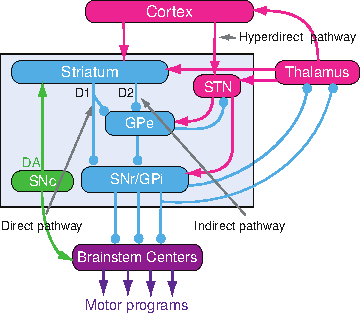
\includegraphics[width=0.7\linewidth]{ch-intro/figures/BGAnatomy}
		\caption[Anatomy of the Basal Ganglia]
		{\textbf{Schematic Anatomy of the basal ganglia.}
		The gray highlighted rectangle depicts the BG nuclei.
		Arrows show anatomical connections (\textit{red}: glutamatergic; \textit{blue}: GABAergic; \textit{green}: DAergic).
		STN:~subthalamic nucleus;
		GPe:~globus pallidus externus;
		SNc:~substantia nigra pars compacta;
		SNr:~substantia nigra pars reticulata;
		GPi:~globus pallidus internus;
		DA:~dopamine.
		Figure slightly modified from~\cite{Grillner2016BG}.
		}
		\label{fig:intro:BGAnatomy}
	\end{center}
\end{figure}


%=============================================================
\subsubsection{Striatum} \label{intro:anatomy:striatum}
%order of material: MSNs > interneurons > topography > DLS/DMS
The striatum is the main input nucleus of the \gls{bg} and one of the largest undivided structures in the rodent brain atlas~\cite{Hintiryan2016NN,Hunnicutt2016}.
Despite having several cell types, GABAergic \glspl{msn} constitute~90--95\% of its neural population.
Their name stems from their morphological appearance, their size and the abundance of their dendritic processes~\cite{TURNER2000BasalFunction}.
\Glspl{msn} receive glutamatergic inputs from the entire cortex, thalamus, and amygdala.
These excitatory afferents make up 80\% of all the synapses in the striatum~\cite{Wilson2007GABAergicNeostriatum}.
Several other inputs modulate the responsiveness of the \glspl{msn} to massive excitatory synapses, namely \gls{da} afferents, inhibitory input from GABAergic interneurons (and from \gls{msn} collaterals), and input from cholinergic interneurons~\cite{Dudman2015Book}.
Consequently, \glspl{msn} are mostly quiescent, except during motor activity or in response to sensory stimuli~\cite{KandelBook2001}.
\par
Based on morphological and neurochemical identification, there are two major types of interneurons within the striatum, which make up~5--10\% of striatal neural population:
    the medium aspiny GABAergic interneurons, and the large aspiny cholinergic interneurons.
The most abundant type of GABAergic interneurons express parvalbumin.
Parvalbumin-positive interneurons are physiologically characterized by their hyperpolarized resting potential and fast spiking activity.
Thus, they are usually referred to as the \glspl{fsi}~\cite{Dudman2015Book}.
They target \glspl{msn} at the soma level by gap junctions and provide powerful GABAergic synapses to several hundreds of surrounding \glspl{msn}~\cite{Grillner2016BG, Gage2010FSI}.
Although they are scarce, with higher firing rate compared to \glspl{msn}, they are capable of delaying action potentials in the neighboring \glspl{msn}~\cite{Wilson2007GABAergicNeostriatum}.
\par
Large cholinergic interneurons are the other type of striatal interneurons.
Their soma could be as large as~40~$\mu$m in diameter, with expansive arborization and an axon that extends over~2~mm~\cite{Dudman2015Book}.
They have tonic discharge patterns, and in primate, are called \textit{tonically active neurons}.
\Glspl{fsi} and cholinergic interneurons are not noticeable in number, nonetheless, they are believed to strongly contribute to the dominance of inhibition in the striatum~\cite{Gage2010FSI}.
In addition to these two, several other types of interneurons within the striatum are described as well~\cite[see][]{Grillner2016BG, Dudman2015Book}.

\paragraph{Organization of Cortical Inputs}
The striatum receives massive input from almost the entire cortex.
It has been long known that corticostriatal projections are topographical, roughly following the rostro-caudal and latero-medial organization of the cerebral cortex.
For instance, frontal cortices project to rostral areas, sensorimotor cortex provides input to \gls{ds}, and parietal cortex to more caudal areas~\cite{Dudman2015Book}.
Such topographical organization suggests parallel circuits for limbic, cognitive, and sensorimotor processes via cortico-\gls{bg}-thalamo-cortical loops~\cite{Alexander1986}.
In this framework, the sensorimotor loop consists of the \gls{dls}, ventrolateral thalamus, and sensorimotor cortices.
Similarly, the limbic (emotional) loop includes the ventral striatum, dorsomedial thalamus, and limbic areas (amygdala, limbic cortices, and hippocampus).
Finally, the cognitive (associative) loop comprises the \gls{dms}, anterior ventral thalamus, and frontal cortices~\cite{Jahanshahi2015NatRevNeurosci}.
However, reduced number of neurons from cortex to \gls{bg} outputs by a factor of more than one million, implies integration of information from different loops to shape the appropriate behavior~\cite{Boraud2018ProgNeurobiol}.
\par
In the \gls{ds}, loose somatotopic organization has also been long reported~\cite[see][as an early review]{Mink1996}.
In \citeyear{Carelli1991}, \citeauthor{Carelli1991} recorded from hundreds of neurons during movement and somatosensory stimulation.
They found that more than 70\% of recorded neurons in the \gls{dls} responded to movement, passive manipulation or cutaneous stimulation.
Moreover, neurons selective for an individual body part (e.g., the forelimb, neck, snout,\dots) were generally located in close proximity, generating a somatotopic map~\cite{Carelli1991}.
Such an anatomical mapping from sensorimotor cortices to the \gls{dls} has recently been quantitatively scrutinized in mice too~\cite{Hunnicutt2016, Hintiryan2016NN}.
These studies, using multiple injections of anterograde tracers, constructed a comprehensive excitatory input map of the \gls{ds}.
\autoref{fig:intro:InputMap} shows an example of different cortical regions projecting to the \gls{dls} in a somatotopic manner.
Interestingly, cluster analysis of cortical regions projecting to arbitrarily-defined striatal voxels revealed dorsal striatal subregions which relatively agreed with parallel circuits for limbic, cognitive, and sensorimotor processes.
With the strictest clustering criteria, \citeauthor{Hunnicutt2016} identified two areas, which map roughly to the \gls{dls} and \gls{dms}\footnotemark~\cite{Hunnicutt2016}.
\footnotetext{
    \Gls{dls} and \gls{dms} correspond to the putamen and caudate nuclei, respectively.
    In primates, the internal capsule divides the striatum in two halves, thus the use of caudate-putamen nucleus instead of the striatum is more common.
    }
\begin{figure}[bth!]
  \begin{center}
    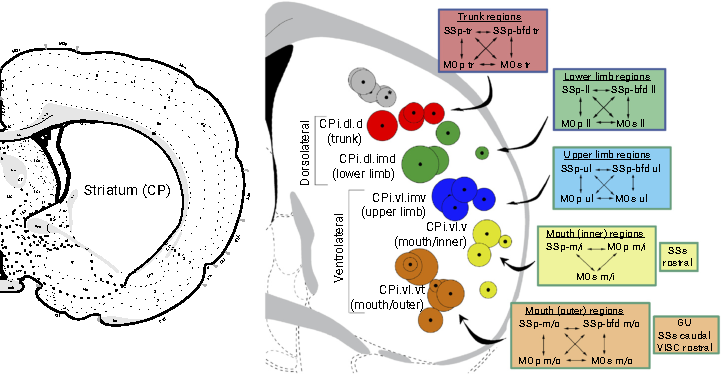
\includegraphics[width=0.9\linewidth]{ch-intro/figures/StriatumInputMap}
    \caption[Somatotopic map of cortical inputs to \gls{dls}]
    {\textbf{Somatotopic map of cortical inputs to \gls{dls}.}
    \textit{Left}: striatum in the rat brain atlas.
    \textit{Right}: input from somatosensory cortices form a topographic map in the \gls{dls}.
    Abbreviations are defined in the original reference and are not important for the purposes of this work.
    Figure adopted from~\cite{Hintiryan2016NN}.
    }
    \label{fig:intro:InputMap}
  \end{center}
\end{figure}
Of note, \gls{dms} and \gls{dls} have been suggested as functionally distinct areas as well, contributing to goal-directed and habitual behaviors, respectively~\cite{Yin2006NatRevNeurosci}.
Another noteworthy result concerns the extent of these areas.
The identified \gls{dls} receives inputs from the motor cortex, somatosensory cortex, but also frontal association cortex, amygdala, and prelimbic cortex.
Importantly, the \gls{dls} expands medially much larger than what has been traditionally regarded as the \gls{dls}, suggesting that areas that has been considered as the \gls{dms} in the literature, partially includes the \gls{dls} too.
It has since been suggested that the sensorimotor information in the \gls{ds} is more prevalent than classically considered and it should be taken into account in studies concerning the function of the striatum~\cite{Robbe2018}.


\paragraph{Direct/Indirect Pathways}
\label{intro:bg:pathways}
\Glspl{msn} are the majority of the neuronal population of the striatum.
They are homogeneously distributed in a way that the striatum lacks any architectural organization when all the neurons are stained in a histologic slice~\cite{Dudman2015Book}.
Nonetheless, \glspl{msn} are divided into two major categories, based on their neurochemistry and connectivity.
One class expresses \gls{d1} and projects directly to \gls{gpi}/\gls{snr} neurons, hence they form the so-called \emph{direct pathway}\!{}.
The second kind expresses \gls{d2} and projects to the \gls{gpe}.
This pathway, in turn, leads to the output nuclei through two routes:~monosynaptic~\gls{gpe}$\rightarrow$output, or bisynaptic~\gls{gpe}$\rightarrow$\gls{stn}$\rightarrow$output projections~\cite{TURNER2000BasalFunction}.
These \glspl{msn} form the \emph{indirect pathway}\!{} (\autoref{fig:intro:BGAnatomy}).
\Gls{d1}-expressing neurons and \gls{d2}-expressing neurons exist in rather equal numbers and are intermingled and spread rather uniformly throughout the striatum~\cite{Dudman2015Book}.
The net effect of the direct pathway activity is to inhibit the \gls{gpi}/\gls{snr} nuclei, thus releasing the target areas of the \gls{bg} from inhibition (i.e., disinhibition).
On the contrary, indirect pathway activity, through \gls{gpe} and \gls{stn}, disinhibits the output nuclei and in turn causes further inhibition of \gls{bg} targets.
This bidirectional control of the \gls{bg} output by the direct and indirect pathways is believed to substantially influence the behavior, either by gating movements~\cite{Kravitz2010Nature}, or by selecting the appropriate actions and repressing others~\cite{Cui2013Nature}.
\par
\Gls{da} significantly modulates neuronal activity in the striatum~\cite{Panigrahi2015Cell}.
\Gls{pd}, with many behavioral and cognitive ramifications, is characterized by the degeneration of \gls{snc} neurons and \gls{da} depletion in the striatum~\cite[see][for a comprehensive review]{McGregor2019Neuron}.
Axons from \gls{snc} neurons arborize widely in the striatum.
They primarily synapse with principle neurons (\glspl{msn}) targeting the narrow necks connecting the spines to dendritic shafts, whereas cortical inputs mostly terminate on dendritic shafts.
This particular arrangement may be a mechanism by which \gls{da} release modulates the cortical input to the \glspl{msn}~\cite{TURNER2000BasalFunction}.
This mechanism is of extra importance since \gls{d1}-expressing neurons are excited by \gls{da}, whereas \gls{d2} neurons are inhibited.
Thus, \gls{da} signals can up-regulate or down-regulate the excitability of the direct and indirect pathways.
\par
The physiology and anatomy of the \gls{bg} give this structure the potential to have a wide range of functions, from providing a central clock by implementing models such as the ramping activity, to controlling actions through different mechanisms, and even providing an essential node in the decision-making network.
Following section reviews the evidence in support of each of these possibilities.


%============================================================
\subsection{Basal Ganglia as a Clock}
\label{ch:intro:BGTime}

Many brain structures have been proposed to contribute to time estimation.
Among them, the \gls{bg} are especially of interest, since they are directly involved in motor processes as well~\cite{KandelBook2001}.
Moreover, the \gls{bg} are also involved in reinforcement learning---selecting actions in an uncertain world in a way that maximizes reward in the long term~\cite{Petter2018}.
Such learning necessitates an understanding of temporal contingencies in order to maximize future rewards.
Behavioral data supports that animals build probabilistic models for timing of the reward and even adjust their models in response to modified reward delays~\cite{li2013PNAS}.
% In general, execution of any complex behavior requires proper timing of the comprising sub-actions.
\par
The \gls{bg} are often implicated in timescales of several hundreds of milliseconds to several seconds~\cite{Paton2018NeuronRev}.
Evidence of involvement of the \gls{bg} in timing stems from a variety of sources, including pathologies such as \gls{pd}, lesion studies, and pharmacological and genetic manipulations.
Following the taxonomy discussed in \autoref{ch:intro:taxonomy}, there is evidence of involvement of the \gls{bg} in sensory timing.
\Citeauthor*{Rao2001} reported encoding of time intervals in the human striatum in a task in which subjects reported whether an interval was shorter or longer than a standard interval of 1200~ms.\footnotemark\
They also observed a dynamic network of cortical activity in inferior parietal, premotor, and dorsolateral prefrontal cortex.
These nodes in the network were attributed to different components of temporal processing, respectively, attention, memory, and interval comparison.
They ultimately concluded the implication of ``striatal dopaminergic neurotransmission in hypothetical internal timekeeping mechanisms''~\cite{Rao2001}.
\footnotetext{
    This paradigm is commonly referred to as ``interval categorization task''.
    }
Moreover, \Citeauthor*{Pouthas2005} investigated interval categorization for two durations (450~ms and 1300~ms).
They observed ramping striatal activity during both intervals.
They concluded a direct role of the basal ganglia in duration estimation, and that the caudate nucleus ``may support a clock mechanism''~\cite{Pouthas2005}.
Similar evidence exists in other species as well.
\Citeauthor*{Gouvea2015Elife} trained rats in a sensory categorization task to judge whether an interval is shorter or longer than 1.5~s.
They decoded animals' choice and elapsed time from ensembles of striatal neuronal activity, whereas apparent behavior in an overhead video failed to do so.
Transient inactivation of the \gls{ds} did impair performance, however, it did not cause a systematic under-- or over--estimation~\cite{Gouvea2015Elife}.
\par
Furthermore, the \gls{bg} are also well studied for their role in motor timing.
\Citeauthor*{Matell2003} trained rats to receive a reward in a fixed interval reinforcement schedule.\footnotemark\
The interval alternated between 10~s (25\% of trials) and 40~s (75\% of trials).
After learning, animals increased their lever press rate around the reinforced intervals.
Electrophysiological recordings from the striatum showed neurons with tuned firing rate only around 10~s interval, but not 40~s, while apparent behavior of the animals was similar.
The authors then suggested that a population of duration-coding cells, each tuned to different values, could accurately represent the elapsed time~\cite{Matell2003}.
\footnotetext{
    In operant conditioning, fixed interval reinforcement schedule refers to a type of conditioning whereby a response is reinforced only if a certain period of time has elapsed.
    }
\Citeauthor*{Mello2015} also used a similar task for intervals ranging between 12~s to 60~s~\cite{Mello2015}.
They found striatal cells that rescaled their activity when intervals changed.
As rats adjusted to the new interval, time estimations decoded form population dynamics predicted animals' timing performance.
In another study, \Citeauthor*{Bakhurin2017JNeuro} used an operant conditioning paradigm in which the conditioned stimulus was followed by a delayed reward delivery (2.5~s after cue onset) and they monitored anticipatory licking of mice as a behavioral readout of temporal perception~\cite{Bakhurin2017JNeuro}.
After training, animals started licking $\sim$1.5~s after the conditioned stimulus.
Simultaneously recorded neurons in the striatum and orbitofrontal cortex displayed sequential activity during the interval.
A machine learning algorithm was then trained to decode the elapsed time from the stimulus onset.
They showed that both striatal and cortical networks ``encoded time, but the striatal network outperformed the orbitofrontal cortex''.
Interestingly, removing the neurons modulated by licking activity from the decoder significantly reduced its performance, however, it still remained higher than the chance level~\cite{Bakhurin2017JNeuro}.
\par
A source of impact in the \glsentrylong{bg} is the neuromodulatory effect of \gls{da}.
\Glsentrylong{da}'s role in reward processing and circuit dynamics of the striatum is discussed in \autoref{intro:BGAnatomy} and \autoref{intro:BGMotor}.
\Gls{da} is also believed to be involved in timing~\cite{Paton2018NeuronRev}.
In a peak interval procedure,\footnotemark\ \Citeauthor*{DeCorte2019} found that \gls{d2} blockade delayed start and stop times for an interval of 6~s.
Whereas, blockade of \glspl{d1} delayed stop times only.
Then they stressed the role of the \gls{ds} in timing, with \gls{da} ``being particularly critical for the temporal control of action''~\cite{DeCorte2019}.
\footnotetext{
    Peak interval procedure is a common task used to study timing.
    Similar to fixed interval schedules, a cue indicates that a response will be reinforced only after a certain period of time has elapsed.
    The profile of the response around the interval is then studied.
    }
\Glsentrylong{da} neurons encode reward prediction errors which requires accurate reward predictions~\cite[see][]{Berke2018NN}.
\Citeauthor*{Takahashi2016} recorded from \gls{da} neurons of rats while they performed a task with uncertainty in reward timing and reward number.
Neuronal activity showed error signals in response to both types of prediction error, however, after ventral striatal lesions, neurons only responded to changes in reward number, and not reward timing.
These results suggested that time-dependent component of reward prediction of \gls{da} neurons might rely on the ventral striatum~\cite{Takahashi2016}.
In an interesting study, \Citeauthor*{Paton2016Sci} measured and manipulated the activity of \gls{da} neurons in a 1.5~s interval categorization task~\cite{Paton2016Sci}.
\Gls{da}ergic activity predicted animal's time estimates.
Transient activation (\textit{inhibition}) of \gls{da} neurons caused under- (\textit{over-}) estimation of the interval.
Hence, the authors concluded that ``\gls{da} neurons, which are so central to reward processing, exert control over time estimation'', although these results reflect \gls{da} function in general, not specifically in the \gls{bg}.
Similar to scaling of spiking activity in the striatum~\cite{Mello2015}, \gls{da} concentration in the \gls{ds} is also scalable to time intervals in several second time range~\cite{Howard2017}.
However, \citeauthor{Howard2017} then conducted a series of experiments and concluded that the \gls{da} signal in the \gls{ds} does not reflect interval timing per~se, rather it is specific to behavioral choice of action~\cite{Howard2017}.
\par
Deficits in temporal perception occur in many disorders.
Since pathologies usually affect multiple brain structures or manifest in several behavioral domains, it is unclear whether timing deficits are responsible for dysfunctions, or they are merely the result of other malfunctioning systems.
Schizophrenia, for example, is a complex psychiatric disorder with a wide range of symptoms, including: delusions, hallucinations, speech poverty, and timing deficits.
Time perception impairment is reported in sensory and motor timing tasks and is associated with increased \gls{da} levels in the striatum, as well as abnormal activity in the dorsolateral prefrontal cortex and supplementary motor area~\cite[see][]{Snowden2019}.
Furthermore, it has been reported that individuals with attention deficit/hyperactivity disorder did not benefit from the temporal predictability in an oculomotor task that displayed a target after a random delay~\cite{Dankner2017}.
Additionally, timing deficiency has also been reported in Huntington’s disease.
Patients demonstrated lower sensitivity to temporal regularities and overall, poorer performance in different types of sensory timing tasks.
Their performance negatively correlated with the progression of Huntington’s disease as well~\cite{Cope2014}.
Finally, \gls{pd} also affects timing performance.
Lower timing performance has been reported in multiple tasks.
\Citeauthor*{Harrington1998} showed that \gls{pd} patients were impaired in sensory timing, in which ``duration perception'' was weaker compared to the control group.
Also, in a motor task, whereby subjects performed finger-tapping synchronized with a series of tones (in the subsecond range), \gls{pd} participants were significantly more variable~\cite{Harrington1998}.
Interestingly, it has been proposed that frequent exposure to temporally-structured tones might alleviate motor symptoms of \gls{pd}, especially gait and stride length~\cite{Dalla2017}.


%============================================================
\subsection{Basal Ganglia as a Motor System}
\label{intro:BGMotor}
{\singlespacing \epigraph{Why do we and other animals have brains?\dots You may reason that we have one to perceive the world or to think, and that is completely wrong\dots We have a brain for one reason and one reason only, and that is to produce adaptable and complex movements.}
{\textit{Daniel Wolpert, TED talk}}}
\noindent
Regardless of whether one agrees with Daniel Wolpert's strong words above or not, the importance of volitional movements is trivial.
The striatum, in particular, is reported to be involved in different aspects of voluntary action.
Among those, its role in motor control\footnotemark\ is well-studied.
\footnotetext{
    By ``motor control'', I refer to the performance/execution of movements or actions.
    Those actions are already part of the subject's motor repertoire, i.e., they have been learned earlier.
}


\subsubsection{Action Selection and Chunking}
The \gls{bg} are postulated to control voluntary actions through direct/indirect pathways.
\Citeauthor{Mink1996} and others proposed the action selection model, according to which the two pathways may work in concert to support the desired actions (direct pathway) and suppress the unwanted competing ones (indirect pathway)~\cite{Mink1996}.
Cell-type specific techniques allowed investigating such a dissection \textit{in-vivo}.
For example, by stimulating \gls{bg} pathways, locomotive activity was bidirectionally controlled~\cite{Kravitz2010Nature}.
Moreover, calcium transients recorded from \gls{d1} and \gls{d2} striatal neurons demonstrated concurrent activity in both cell types during movement~\cite{Cui2013Nature,Barbera2016Neuron}.
Interestingly, \gls{msn} ensembles that were active during specific actions were generally spatially closer together and more correlated between similar actions~\cite{Klaus2017Neuron}.
These studies, however, found similar patterns in both \gls{d1} and \gls{d2} neurons.
Therefore, they proposed a revised action selection model in which the indirect pathway might not inhibit all the competing actions, rather exert a more specific control over particular aspects of an action~\cite{Klaus2017Neuron}.
Accordingly, during the execution of a learned lever pressing sequence, some neurons displayed sustained activity during the sequence in both direct and indirect pathways, while some favored the start and stop of the sequence~\cite{Jin2014NN}.
\par
Related to the action selection hypothesis is chunking patterns observed predominantly in the \gls{dls}.
Striatal neurons, in a wide variety of tasks, have preferential firing around the boundaries of a learned motor sequence.
For instance, \Citeauthor{Barnes2005Nature} showed that \glspl{msn} in the \gls{dls} fired sharply at the start and end of an overlearned run bout in a T-maze~\cite{Barnes2005Nature}.
This chunking of a behavioral sequence was then proposed to mediate the process of acquiring motor habits.
In another study, mice were trained to press a lever 8 times to receive a reward (fixed-ratio schedule)~\cite{Jin2010N}.
After training, mice pressed the lever in close succession.
Next, authors recorded the spiking activity of \gls{dls} neurons and reported that the firing of many neurons peaked just before the first press or around the last one.
This pattern grew stronger with learning~\cite{Jin2010N}.
Moreover, \Citeauthor{Martiros2018} trained rats to each perform a unique lever pressing sequence (first rat: lever 1$\rightarrow$1$\rightarrow$2; second rat: lever 2$\rightarrow$1$\rightarrow$2)~\cite{Martiros2018}.
After learning, similar ``sequence-bracketing'' activity was recorded in the \gls{dls}, but only for the reinforced sequence of each animal, and not for the non-reinforced sequences which were rewarded for other subjects.
\par
Further experiments indicated that the activity profile of \glspl{msn} during movement is more complex.
There is now evidence indicating that the striatal activity may form a continuous space, and functional clusters may reflect instantaneous movement information, rather than discrete start and stop signals~\cite{Sales-Carbonell2018, Markowitz2018Cell}.
\Citeauthor{Markowitz2018Cell} decoded subsecond syllables of ongoing behavior using both the \gls{d1} and \gls{d2} activity~\cite{Markowitz2018Cell}.
\Citeauthor{Sales-Carbonell2018} trained head-fixed mice to run uninterruptedly for 100~cm on a wheel and then remain immobile to allow the next trial to start~\cite{Sales-Carbonell2018}.
Recording from striatal \glspl{msn} in proficient animals showed that neuronal activity is modulated during the entire running phase, including the start and stop points.
Statistical analysis of neuronal activity indicated a continuous representation of the run phase in the striatum.
Finally, authors suggested that the over-representation of the start/stop of the run phase may be due to the altered sensorimotor state that occurred at those points, such as licking the reward or changing the locomotion speed~\cite{Sales-Carbonell2018}.


\subsubsection{Kinematics and Urgency}
Control of movements has been associated with the \gls{bg} for a long time.
This link dates back to the first descriptions of the behavioral deficits of \gls{pd} patients by James Parkinson in 1817.
% \Gls{pd} is characterized by loss of \gls{snc} neurons and their ascending projections to the striatum.
Tetriakoff, in 1919, performed postmortem analysis of the brains of patients diagnosed with \gls{pd}, and first reported loss of dark-pigmented nigral neurons.
Ever since, motor dysfunctions of \gls{pd} are believed to be due to \gls{da} depletion in the striatum~\cite{Hornykiewicz2006,McGregor2019Neuron,Redgrave2010, Panigrahi2015Cell}.
\par
Although symptoms differ from patient to patient, three behavioral deficits are typical for \gls{pd}:
    resting tremor, which is the most apparent;
    rigidity and stiffness of muscles;
    and bradykinesia, i.e., reduced movement vigor.
Reduced vigor in \gls{pd} has been investigated to distinguish between the speed/accuracy trade-off and energetic cost as two possible determinants of movement speed.
\Citeauthor{Mazzoni2007} asked \gls{pd} patients and age-matched control subjects to make self-paced arm movements as accurate as possible toward a target with a speed within an explicitly requested range~\cite{Mazzoni2007}.
After 20 successful trials, the required speed range and/or target distance changed to the next experimental condition.
Both groups of subjects, across all conditions (3~target distances, 4~speed ranges) achieved similar peak velocities and maintained the same level of accuracy.
However, patients needed significantly more trials to reach the criterion to advance to the next condition.
Analysis of those extra trials performed by the \gls{pd} patients demonstrated that they used a higher proportion of slower movements while retaining the speed range the same as control subjects.
Moreover, authors showed that the number of trials required to reach the criterion, as a measure of task difficulty, strongly correlated with subjects' average acceleration.
This linear contribution (denoted as $S_N$) was steeper for control subjects.
In other words, for any given difficulty of the task, \gls{pd} patients \textit{chose} a lower level of acceleration.
Similar linear relationship existed between number of trials to criterion and accuracy as well, but it was the same for control subjects and patient.
Thus, lower $S_N$ in \gls{pd} was not caused by a different speed/accuracy trade-off, rather by another component of task difficulty related to the acceleration.
Authors then argue that acceleration also represents movement energy cost, and that \gls{pd} patients are more sensitive to energy expenditure.
These results suggest that \gls{snc} innervation of the striatum carries a ``motor motivation'' signal and lack thereof in \gls{pd} leads to a propensity for slow movements~\cite{Mazzoni2007}.
Similar results have been reported from patients with pallidal and striatopallidal lesions.
They could generate normal grip force when explicitly instructed, however once left to their own, they failed to squeeze harder to earn more monetary compensation~\cite{Schmidt2008Brain}.
\par
Available methods in animal research provide an opportunity to further dissect the \gls{bg} circuit.
For instance, infusion of the GABA\textsubscript{A} agonist, muscimol, transiently inactivates the surrounding neurons, allowing the researcher to study the functional relevance of the targeted structure.\footnotemark\
\Citeauthor{Desmurget2010JNeurosci} took advantage of this technique to acutely inactivate the sensorimotor territory of the \gls{gpi} in monkeys~\cite{Desmurget2010JNeurosci}.
Monkeys were trained to move a cursor using a joystick to a peripheral target and then move it back to its original position.
The two experimental conditions differed in the degree to which successive target positions were predictable:
    random positioning of the target in each trial;
    or a fixed repetitive sequence of four target positions.
\Gls{gpi} inactivation after overlearning the sequence did not prevent its execution, thus failing to support a role for the \gls{bg} in ``storage or execution of well learned motor habits''.
The main impairment observed post-injection was reduced movement speed and amplitude in both conditions, i.e., random sequences and the overlearned sequence.
Thus, they concluded that the motor circuit of the \gls{bg} contributes to the kinematics of motor execution but not its production nor storage of learned sequences~\cite{Desmurget2010JNeurosci}.
\footnotetext{
    This technical approach is not free from skepticism.
    \Citeauthor{Otchy2015Nature} present convincing evidence that acute circuit manipulations, such as inactivation, have unintended consequences.
    In a complex dynamical system such as the brain, by transiently changing the activity of the area of interest, off-target downstream structures are driven into an unnatural state that could have behavioral implications of its own~\cite{Otchy2015Nature}.
    }
In general, reduced vigor is the most common phenomenon in conditions of perturbed \gls{bg} activity~\cite{Bailey2006JNeurosci, Rueda2015NN, CastaneAnna2010, Bergstrom2018Cell, Lemke2019NN, Geddes2018Cell, Bailey2006JNeurosci, Hart2018CurrBiol}.
Importantly, in many types of tasks, including the two mentioned above, reduced vigor could also be regarded as an overestimation of the cost action, i.e., a conservative policy in energy expenditure.
\par
% add a linking sentence
% Decision-making is another example of relevance of 
Decision making is another front where cost evaluation is essential.
Many decisions are based on partial information that has been gathered over time, like deciding whether the approaching animal is a predator or a prey, or choosing the \textit{best} restaurant for dinner~\cite{Bogacz2010TINS}.
In such cases, one faces a dilemma analogous to the speed/accuracy trade-off in motor control: waiting longer to accumulate information makes for better decisions at the cost of diminishing reward, increasing danger, and the passage of time.
The \gls{bg} are implicated in controlling this trade-off in decision-making.
In an interesting paper, \citeauthor{Thura2017Neruon} used a task that allowed dissociating different aspects of decision-making and movement control~\cite{Thura2017Neruon}.
They extensively trained monkeys to guess which of the two potential targets would receive the majority of the tokens that jumped from a central point to one of the possible targets every 200~ms.
Crucially, after the subject reached the target, the rest of the tokens jumped more quickly, thus presenting the monkey with a trade-off to either make confident decisions or guess earlier and receive potential rewards sooner.
How much faster the tokens jumped after the decision (every 150~ms, or every 50~ms), compared to their normal pace (every 200~ms) determined different speed/accuracy trade-off policies---the faster they jumped, the more hasty decisions were justified.
They performed electrophysiological recordings in behaving animals from the motor and premotor areas as well as the \gls{gpi} and \gls{gpe}.
They showed that during deliberation, information about selecting a target existed in the motor areas, but it was much weaker in the \gls{bg} output.
They observed ramping activity in the \gls{gpi} that ``invigorate[s] the decision-making process by providing an urgency signal''.
This urgency signal grew over time and and was adjusted to different speed/accuracy trade-off policies, but did not reflect the amount of evidence or the target chosen by the animal~\cite{Thura2017Neruon}.
In the condition wherein tokens jumped the fastest post-decision, unsurprisingly, the ratio of hasty decisions increased.
Moreover, the animals made faster movements too~\cite{Thura2014JNeurosci}.
% This suggests a common underlying mechanism that relates to motivation, reward expectancy and movement kinematics.
Therefore, the urgency signal may act as a determinant of the timing of decisions and the vigor with which those decisions are implemented into actions in pursuit of maximal reward~\cite{Carland2019NeuroSci}.
\par
Neural activity in the striatum has been shown to encode kinematics of ongoing behavior too.
Single \gls{dls} neurons of rats encode locomotion speed and acceleration~\cite{Rueda2015NN}.
In addition, \gls{d1} and \gls{d2} population activity was correlated with locomotion speed in mice~\cite{Barbera2016Neuron}.
Moreover, simultaneous recording of calcium activity and mouse 3-D exploratory behavior showed that direct (\textit{indirect}) pathway activity correlated (\textit{anti-correlated}) with movement velocity.
Nonetheless, ongoing kinematics was best decoded from the activity of both pathways, suggesting that they contain non-redundant information~\cite{Markowitz2018Cell}.
\par
Contrary to the classic model of the \gls{bg}, in which the direct pathway activity is prokinetic and the indirect pathway activity inhibits movement~\cite{Kravitz2010Nature}, and to the action selection model of the \gls{bg} that proposes that the direct pathway promotes the selected action while the indirect pathway concurrently suppresses the competing actions~\cite{Cui2013Nature}, a novel behavioral paradigm revealed that control of movement velocity might be the underlying mechanism implemented by the \gls{bg}.
\Citeauthor{Yttri2016Nature} in an article that is one of my all-time favorites, trained head-fixed mice to perform self-paced forelimb movements to obtain a delayed water reward~\cite{Yttri2016Nature}.
While all movements bigger than an easy-to-reach threshold were rewarded, the fastest ones were detected early after initiation and the fastest third of the movements triggered a photo-stimulation of either \gls{d1} or \gls{d2} neurons in the \gls{dms}.
Brief stimulation of direct pathway \glspl{msn} produced a significant increase in movement velocity that sustained for multiple trials after cessation of stimulation.
On the contrary, indirect pathway stimulation reduced the movement vigor.
Interestingly, stimulating the slowest, rather than the fastest, third of trials generated the opposite effect:
\gls{d1} activation reduced and \gls{d2} activation increased the velocity.
In all cases, other movement parameters, such as amplitude, duration and tortuosity remained unchanged.
Thus, activating the \glspl{msn} was sufficient to produce bidirectional control of movement velocity.
% This control, however, was eliminated following the administration of a \gls{da} antagonist, suggesting an explicit interaction between the \gls{da} input, carrying a reward signal, and the activation of \glspl{msn} in the striatum.
The authors then argued that reinforcement learning models of the \gls{bg} could not readily act on a continuous kinematic parameter of movement and they proposed an algorithmic learning rule in which a signed pathway-specific signal determines the mean velocity of movement while a homeostatic component opposes the learned changes in velocity.
Such a learning rule explained the empirical data and was conceptually predicted by a \gls{hdg} model of the \gls{bg}~\cite{Yttri2016Nature, Yttri2018MovDisorder}.
The \gls{hdg} model describes movement vigor as a function of both descending motor commands from the cortex and the \gls{bg} output.
The \gls{bg} in this model applies a causal gain to the kinematics of behavior~\cite{Yttri2018MovDisorder}.
This gain is determined by the relative strengths of cortical synapses onto \gls{d1} and \gls{d2} neurons.
Synaptic strengths depend on the plasticity mediated by prior activity and the \gls{da}, which in turn represents a recent history of reward.
Thus, the bidirectional control of vigor by either pathway is due to the altered relative synaptic weights of \gls{d1}/\gls{d2} neurons upon stimulation~\cite{Yttri2016Nature}.
The \Gls{hdg} model predicts that stimulating random trials, stimulating every trial, and suppressing \gls{da}-mediated plasticity should abolish control of vigor.
All of these predictions were empirically verified~\cite{Yttri2016Nature}.
\par
Related to the \gls{hdg} model discussed above,~\citeauthor{Dunovan2016FrontNeurosci} proposed a model in which the \gls{bg} encode action uncertainty through direct-indirect pathway competition~\cite{Dunovan2016FrontNeurosci}.
This competition implements a commitment to action algorithm by comparing the activity of the direct pathway to the indirect pathway.
Due to the heavily inhibited default state of the \gls{bg}, the commitment to action only happens if the direct pathway provides enough evidence, otherwise no action is executed.
Sensory and contextual evidence is provided by the weighted corticostriatal inputs that modulate direct/indirect pathway activity~\cite{Dunovan2016FrontNeurosci}.
The ratio of \gls{d1}/\gls{d2} activity determines the outcome of the competition, the time point at which the action is committed, and possibly, the vigor with which it is executed.